\documentclass[twocolumn]{article}
\usepackage{graphicx}
\usepackage{fullpage}
\usepackage{amssymb}
\usepackage{amsmath}
\usepackage{listings}
\usepackage{color}

\definecolor{dkgreen}{rgb}{0,0.6,0}
\definecolor{gray}{rgb}{0.5,0.5,0.5}
\definecolor{mauve}{rgb}{0.58,0,0.82}

\lstset{frame=tb,
    language=C,
    aboveskip=3mm,
    belowskip=3mm,
    showstringspaces=false,
    columns=flexible,
    basicstyle={\small\ttfamily},
    numberstyle=\tiny\color{gray},
    keywordstyle=\color{mauve},
    commentstyle=\color{dkgreen},
    stringstyle=\color{green},
    breaklines=true,
    breakatwhitespace=true,
    tabsize=3
}

\title{\textbf{The exponential function}}
\author{Niels Munch Mikkelsen}

\begin{document}
    \maketitle

    \section{Introduction}
    The real exponential function $\exp(x): \mathbb{R}\rightarrow\mathbb{R}$ is defined as the power series
    \begin{equation}\label{eq:power}
    \exp(x) = \sum_{n=0}^\infty \frac{x^n}{n!} \;.
    \end{equation}
    This function has the special property that it is its own derivative, making it important in many areas of mathematics and the sciences.

    \section{Numerical approximation}
    As a numerical approximation, we use the following code:

    \begin{lstlisting}
#include <math.h>
double exponential(double x)
{
    if (x < 0)
    {
        double result = 1.0 / exponential(-x);
        return result;
    }
    if (x > 1./8)
    {
        double result = pow(exponential(x/2),2);
        return result;
    }
    double result = 1+x*(1+x/2*(1+x/3*(1+x/4
    *(1+x/5*(1+x/6*(1+x/7*(1+x/8
    *(1+x/9*(1+x/10)))))))));
    return result;
}
    \end{lstlisting}
    The input is a double valued parameter x. Before anything is done to the input, we check for negative inputs. If negative inputs are encountered, we recursively return the inverse of the function value, with a changed sign.
    Since the numerical approximation is a finite Taylor series around zero, it will be most accurate for small values. We therefore also check the size of the input. If the value is large, we recursively square the exponential function while dividing the input by two. This will leave the exponential function unchanged, but will ensure that the input is arbitrarily small due to the recursive condition.
    The final computation does not use exponents, but instead repeated multiplication of the value onto itself. The time complexity of this is very low so it is fast to use. We also avoid factorial function that could introduce larger numbers that might give small precision.

    \section{Figures}
    Illustration of the numerical implementation described above can be seen in figure~(\ref{fig:pyxplot}).


    \begin{figure}[h]
        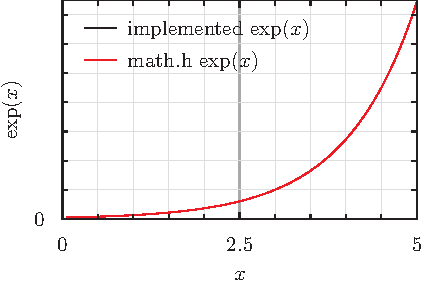
\includegraphics{exponentialPlot.pdf}
        \caption{ Plot of numerical implementation , versus the standard implementation found in the header math.h..}
        \label{fig:pyxplot}
    \end{figure}


\end{document}